% Use only LaTeX2e, calling the article.cls class and 12-point type.

\documentclass[12pt,a4paper]{article}

\usepackage[english]{babel}
\usepackage[utf8]{inputenc}
\usepackage[parfill]{parskip}
\usepackage{textcomp}
\usepackage{hyperref}

\usepackage{listings}
\usepackage{color}
\usepackage{graphicx}
\usepackage{lscape}

% Include your paper's title here

\title{IBMCNX Scripting Documentation} 

\author
{Christoph Stöttner\\
\normalsize{E-mail:  christoph.stoettner@stoeps.de}\\
\normalsize{Blog: http://www.stoeps.de}
}

\lstset{language=python}
\date{}

\begin{document} 

% Make the title.

\maketitle 

\begin{abstract}
    This document is the main documentation of the ibmcnxscripting project. You find tips around jython and how you can create your own scripts for IBM\textsuperscript{\textregistered} Connections and IBM\textsuperscript{\textregistered} WebSphere\textsuperscript{\textregistered} Application Server Administration.
\end{abstract}

\pagenumbering{Roman}
\newpage
\tableofcontents
\newpage
\pagenumbering{arabic}

\section{Jython}

Jython is the Java implementation of Python. I think it is easy to learn and very powerful! 

Jython and Python are interpreting languages and you can test your code in the Jython console or wsadmin. Start Jython and type your code, easy to test and you will get fast results.

There are some good online resources and books to learn the basics of Jython or Python:

\subsection{Learning Resources}

\subsubsection{Online materials}

\paragraph{Online Learning (Python)}

You can use Python learning materials for your first steps! It is very similar to learn Jython.

\begin{itemize}
	\item \url{ http://www.codecademy.com/}
	\item \url{http://learnpythonthehardway.org/book/}
\end{itemize}

\paragraph{Reference}

\begin{itemize}
	\item\url{http://www.jython.org/jythonbook/en/1.0/}
	\item \url{http://www.jython.org/docs/index.html}
\end{itemize}

\subsubsection{Books}

WebSphere Application Server Administration Using Jython (2009)\\
Authors: Robert A. Gibson, Arthur Kevin McGrath and Noel J. Bergman

The Definitive Guide to Jython: Python for the Java Platform (2010)\\
Authors: Josh Juneau, Frank Wierzbicki, Leo Soto and Victor Ng

\subsection{Language elements}

Grouping in Jython is done with an indention of four spaces! Please do not use tab, because i had several issues with code errors on Windows, when i have used tab grouping.

\subsubsection{Comments}

Comments in Jython start with \# and all text after this sign will be ignored!

\subsubsection{Variables}

\begin{lstlisting}[style=Python]
# Defining a String
x = 'Hello World'
x = "Hello World Two"
 
#  Defining an integer
y = 10
 
#  Float
z = 8.75
 
# Complex
i = 1 + 8.07j
 
# Multiple assignment
x, y, z = 1, 2, 3
\end{lstlisting}

\subsubsection{Ranges}

\begin{lstlisting}[style=Python]
wsadmin>range(7)
[0, 1, 2, 3, 4, 5, 6]
 
# Include a step in the range
wsadmin>range(0,10,3)
[0, 3, 6, 9]
 
# Good base for loops
wsadmin>range(1,11)
[1, 2, 3, 4, 5, 6, 7, 8, 9, 10]
 
wsadmin>range(20,27)
[20, 21, 22, 23, 24, 25, 26]
\end{lstlisting}

\subsubsection{Lists}

\begin{lstlisting}[style=Python]
#List
wsadmin>dbs = ['activities','blogs','communities','dogear']
wsadmin>dbs[1]
'blogs'
\end{lstlisting}

\subsubsection{Dictionaries}
\begin{lstlisting}[style=Python]
# Dictionary with Performance Data
wsadmin>minConnections = {'activities':1,'blogs':1}
wsadmin>maxConnections = {'activities':50,'blogs':250}
wsadmin>maxConnections
{'activities': 50, 'blogs': 250}
wsadmin>maxConnections.keys()
['activities', 'blogs']
wsadmin>maxConnections.values()
[50, 250]
wsadmin>maxConnections['blogs']
250
\end{lstlisting}

\subsubsection{if - elif - else}

\textbf{Remember:} Grouping of elements is done with an indent of 4 spaces!

\begin{lstlisting}[style=Python]
# Basic
if condition :
    # print or do something
elif other condition :
    # print or do something other
else :
    # print or do completely different
\end{lstlisting}

\begin{lstlisting}[style=Python]
# Example
if value.find( 'CLFWY0217E' ) > -1 :
    print "\t\tuser already converted"
elif value.find( 'CLFWY0212E' ) > -1 :
    print "\t\tuser not found in database"
elif value.find( ' CLFWY0209E' ) > -1 :
    print "\t\tnew identifier '" + data[1] + "' does not exist."
else :
    print '\t\tException value: ' + value
\end{lstlisting}

\subsubsection{Errorhandling}

You can catch errors with try and except.

\begin{lstlisting}[style=python]
try:
    # perform some commands which can raise an exception
except Exception, value:
    # perform exception handling
finally: 
    # perform task which must always be completed
\end{lstlisting}

\section{WebSphere Application Server}

After installing IBM Connections lots of configuration must be done through ISC (Integrated Solution Console). ISC is a good GUI with lots menus and sometimes long click paths. Configuration is possible through \texttt{wsadmin} too, but it is hard to find the necessary commands.

\subsection{Console Preferences}

\subsection{wsadmin}

Long casesensitiv commands with mostly casesensitiv parameters. Hard to remember and on Linux\textsuperscript{\textregistered} no history to recall commands.

Always start \texttt{wsadmin} in \lstinline[style=BashInputStyle]{WAS_HOME/profiles/Dmgr01/bin}! 

\subsubsection{Start wsadmin}

\paragraph{Windows\textsuperscript{\textregistered}:}

\lstinline[style=command.com]{wsadmin.bat -lang jython -username wasadmin -password password}

\paragraph{Linux and AIX\textsuperscript{\textregistered}:}

\lstinline[style=BashInputStyle]{./wsadmin.sh -lang jython -username wasadmin -password password}

\subsubsection{wsadmin set jython as default language}

You can set the default language which is used with wsadmin, so you can save some character in typing.

\begin{lstlisting}[style=BashInputStyle]
edit WAS_HOME/profiles/Dmgr01/properties/wsadmin.properties
\end{lstlisting}

\paragraph{Default:}

\texttt{com.ibm.ws.scripting.defaultLang=JACL}

\paragraph{Set Jyton:}

\texttt{com.ibm.ws.scripting.defaultLang=jython}

\subsection{Wsadmin commands}

There are five management objects within wsadmin. These objects group the commands to the different MBean Servers.

\begin{itemize}
\item AdminConfig
\item AdminApp
\item AdminTask
\item AdminControl
\item Help
\end{itemize}

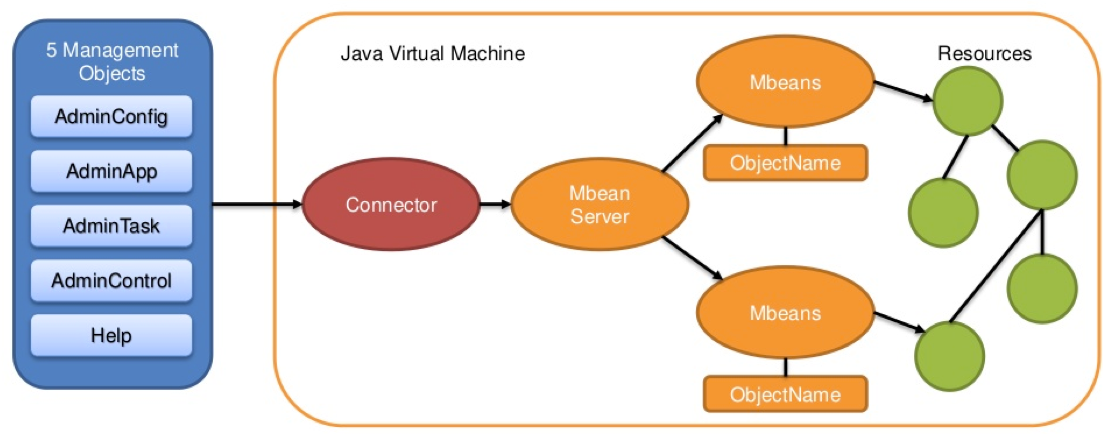
\includegraphics[keepaspectratio=true,width=\textwidth]{wsadmin-objects.png}

\subsubsection{AdminApp Object}

Use the AdminApp object to
\begin{itemize}
\item Installing and uninstalling applications
\item Listing applications
\item Editing applications or modules
\end{itemize}

\paragraph{Examples}

\begin{itemize}
\item List of all applications
	\begin{itemize}
		\item \lstinline{print AdminApp.list()}
		\item \lstinline{AdminApp.list()}
		\item \lstinline{list=AdminApp.list().split('\n')}
	\end{itemize}
\item Change options of applications
	\begin{itemize}
		\item \lstinline{AdminApp.edit('appname',['options'])}
	\end{itemize}
\end{itemize}

\subsubsection{AdminConfig}
\begin{itemize}
\item manage the configuration information that is stored in the repository
\item Example change min- and maxConnections of the DataSource Blogs
\end{itemize}
\begin{landscape}
\begin{lstlisting}
wsadmin>AdminConfig.getid('/DataSource:blogs/') 
'blogs(cells/cnxwas1Cell01|resources.xml#DataSource_1371479885975)'
wsadmin>dataSource1=AdminConfig.getid('/DataSource:blogs/')
wsadmin>print AdminConfig.show(dataSource1)
[authDataAlias blogsJAASAuth]
[authMechanismPreference BASIC_PASSWORD]
[connectionPool (cells/cnxwas1Cell01|resources.xml#ConnectionPool_1384252180672)] 
    [datasourceHelperClassname com.ibm.websphere.rsadapter.DB2UniversalDataStoreHelper] 
    [description "Blogs DB2 DataSource"]
[...]
[jndiName jdbc/rollerdb]
[name blogs]
[...]
[provider blogsJDBC(cells/cnxwas1Cell01|resources.xml#JDBCProvider_1371479882710)] 
    [providerType "DB2 Universal JDBC Driver Provider"]
[statementCacheSize 100]
wsadmin>AdminConfig.modify( dataSource1, '[[statementCacheSize 50]]')
''
wsadmin>AdminConfig.modify( dataSource1, '[[connectionPool [[minConnections 10]
    [maxConnections 100]]]]' )
''
wsadmin>AdminConfig.save()
''
\end{lstlisting}
\end{landscape}
\section{IBM Connections wsadmin commands}

Each application need its own commands:

\texttt{execfile("connectionsConfig.py")}\\
\texttt{execfile("activitiesAdmin.py")}\\
...

\subsection{Load all administrative commands on startup}

Please be careful, when you use this tip, because in multicluster environments, each execfile("appnameAdmin.py") will ask you to select a node, where it will run.

You can create a script with all commands for preloading:

\texttt{loadAll.py:}

\begin{lstlisting}
	execfile('connectionsConfig.py')
	execfile("activitiesAdmin.py")
	execfile("blogsAdmin.py")
	execfile("communitiesAdmin.py")
	execfile("dogearAdmin.py")
	execfile("filesAdmin.py")
	execfile("forumsAdmin.py")
	execfile("homepageAdmin.py")
	execfile("newsAdmin.py")
	execfile("profilesAdmin.py")
	execfile("wikisAdmin.py")
\end{lstlisting}

Load this script at wsadmin startup:\\
\lstinline{./wsadmin.sh -lang jython -profile loadAll.py}

\appendix 

\section{Linux Bash Goodies}
\begin{landscape}
\subsection{.bashrc}

\begin{lstlisting}

# Insert ulimit for file limit 
ulimit -n 64000 
# set WAS_HOME
export WAS_HOME=/opt/IBM/WebSphere/AppServer
# set profileNames
dmgrProfile=Dmgr01
appSrvProfile=AppSrv01
alias dmgrBin='cd $WAS_HOME/profiles/$dmgrProfile/bin' 
alias wsadmin='cd $WAS_HOME/profiles/$dmgrProfile/bin;./wsadmin.sh -lang jython' 
alias nodeBin='cd $WAS_HOME/profiles/$appSrvProfile/bin'  
alias startNode='$WAS_HOME/profiles/$appSrvProfile/bin/startNode.sh'  
alias startDmgr='$WAS_HOME/bin/startManager.sh' 
alias stopNode='$WAS_HOME/profiles/$appSrvProfile/bin/stopNode.sh'  
alias stopDmgr='$WAS_HOME/bin/stopManager.sh' 
alias nodeLog='tail -f $WAS_HOME/profiles/$appSrvProfile/logs/nodeagent/SystemOut.log' 
alias InfraLog='tail -f $WAS_HOME/profiles/$appSrvProfile/logs/InfraCluster_server1/SystemOut.log' 
alias Cluster1Log='tail -f $WAS_HOME/profiles/$appSrvProfile/logs/Cluster1_server1/SystemOut.log' 
alias Cluster2Log='tail -f $WAS_HOME/profiles/$appSrvProfile/logs/Cluster2_server1/SystemOut.log' 

\end{lstlisting}

\end{landscape}
\end{document}
